\documentclass[a4paper, 11pt]{book}
\usepackage{/home/nicolas/Documents/Enseignement/Prepa/bpep/fichiers_utiles/preambule}

\newcommand{\dsNB}{12}
\makeatletter
\renewcommand{\@chapapp}{Kh\^olles MPSI3 -- semaine \dsNB}
\makeatother

% \toggletrue{corrige}  % décommenter pour passer en mode corrigé
\def\w{\omega}\def\O{\Omega} \def\Of{\vv{\O}}
\def\jj{\mathrm{j}}
\def\Hu{\ul{H}}
\def\Uu{\ul{U}}
\def\Iu{\ul{I}}
\def\Zu{\ul{Z}}
\def\Yu{\ul{Y}}
\def\Xu{\ul{X}}
\def\jlw{\jj L\w}
\def\jcw{\jj L\w}

\begin{document}

\chapter{Sujet 1\siCorrige{\!\!-- corrig\'e}}
\section{Question de cours}
\begin{NCexem}[]{Exercice}
    On considère le circuit ci-contre, avec $R = \SI{1.0}{k\Omega}$ et $L =
    \SI{10}{mH}$, donnant le diagramme de \textsc{Bode} ci-dessous~:

    \begin{minipage}{0.60\linewidth}
        \begin{enumerate}
            \item Sans utiliser le diagramme de \textsc{Bode}, quelle est la
                nature du filtre~?
            \item Déterminer sa fonction de transfert et l'écrire sous la forme
                \[\ul{H}(\jj\w) = H_0 \frac{\jj\dfrac{\w}{\w_c}}{1 +
                \jj\dfrac{\w}{\w_c}}\] avec $H_0$ et $\w_c$ des constantes à
                préciser.
            \item On considère une tension d'entrée $u_e(t)$ somme de 3
                harmoniques de mêmes amplitudes, de mêmes phases initiales, mais
                de fréquences respectives $f_1 = \SI{100}{Hz}$, $f_2 =
                \SI{1}{kHz}$ et $f_3 = \SI{100}{kHz}$. Donner le spectre de
                sortie.
        \end{enumerate}
    \end{minipage}
    \hfill
    \begin{minipage}{0.35\linewidth}
        \begin{center}
            \hspace{10pt}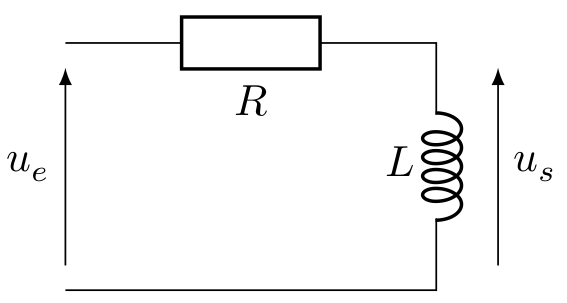
\includegraphics[width=\linewidth]{../../figures/ch12/filtrebob_plain}
        \end{center}
        \begin{center}
            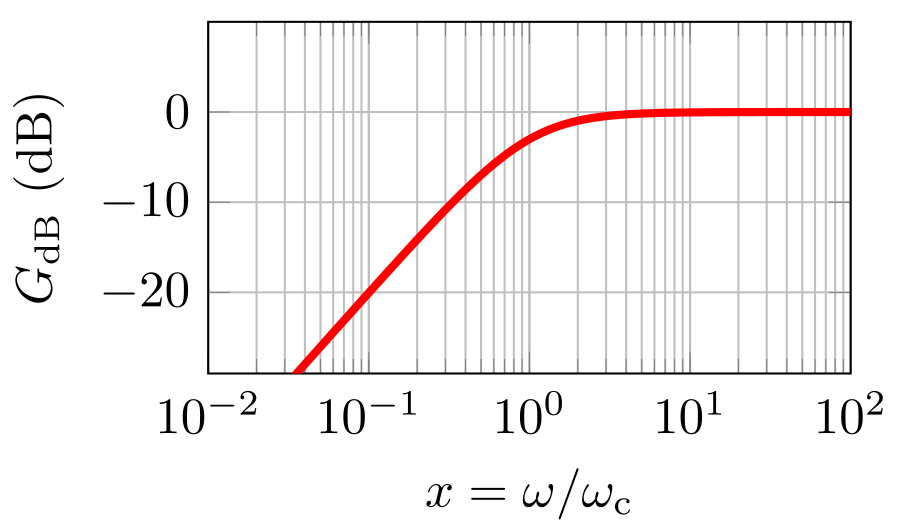
\includegraphics[width=\linewidth]{../../figures/ch12/filtrebob_bode}
        \end{center}
    \end{minipage}
\end{NCexem}

\resetQ
\subimport{/home/nicolas/Documents/Enseignement/Prepa/bpep/exercices/Colle/filtre_passe_haut_ordre_2/}{sujet.tex}

\resetQ
\newpage

\chapter{Sujet 2\siCorrige{\!\!-- corrigé}}
\section{Question de cours}

Comportements intégrateur et dérivateur~: définir les comportements intégrateur
et dérivateur d'un filtre, donner les formes canoniques des filtres passe-bas et
passe-haut d'ordre 1, et démontrer leur comportement intégrateur ou dérivateur.

\subimport{/home/nicolas/Documents/Enseignement/Prepa/bpep/exercices/TD/diagramme_Bode_composition/}{sujet.tex}

\resetQ
\newpage

\chapter{Sujet 3\siCorrige{\!\!-- corrigé}}
\section{Question de cours}

Filtre passe-bande d'ordre 2, RLC série sur R~: présenter le système réel, le
système en RSF complexe, déterminer sa fonction de transfert, son gain en
décibels, l'évolution de sa phase et tracer son diagramme de \textsc{Bode} en
détaillant les asymptotes à basses et hautes fréquences pour le gain.

\subimport{/home/nicolas/Documents/Enseignement/Prepa/bpep/exercices/TD/filtre_RL/}{sujet.tex}
\subimport{/home/nicolas/Documents/Enseignement/Prepa/bpep/exercices/Colle/circuit_RLC_resonance/}{sujet.tex}

\end{document}
